 % --------------------------------------------------------------
% Based on a homework template by Dana Ernst (MTH320 Homework
% template on Overleaf).
% --------------------------------------------------------------

\documentclass[12pt]{article}

\usepackage{graphicx}
\graphicspath{{./images/}}
\usepackage[margin=1in]{geometry} 
\usepackage{amsmath,amsthm,amssymb}
\usepackage{mathdots}
% https://tex.stackexchange.com/questions/146306/how-to-make-horizontal-lists
\usepackage[inline]{enumitem} % allows using letters in enumerate list environment
\usepackage[mathscr]{euscript}
% source: https://stackoverflow.com/questions/3175105/inserting-code-in-this-latex-document-with-indentation

\usepackage{listings}
\usepackage{color}
\usepackage{hyperref}

\newtheorem{theorem}{Theorem}

\definecolor{dkgreen}{rgb}{0,0.6,0}
\definecolor{gray}{rgb}{0.5,0.5,0.5}
\definecolor{mauve}{rgb}{0.58,0,0.82}

\lstset{frame=tb,
	language=C, % language for code listing
	aboveskip=3mm,
	belowskip=3mm,
	showstringspaces=false,
	columns=flexible,
	basicstyle={\small\ttfamily},
	numbers=none,
	numberstyle=\tiny\color{gray},
	keywordstyle=\color{blue},
	commentstyle=\color{dkgreen},
	stringstyle=\color{mauve},
	breaklines=true,
	breakatwhitespace=true,
	tabsize=4
}

\newcommand{\N}{\mathbb{N}}
\newcommand{\Z}{\mathbb{Z}}

\newenvironment{ex}[2][Exercise]{\begin{trivlist}
		\item[\hskip \labelsep {\bfseries #1}\hskip \labelsep {\bfseries #2.}]}{\end{trivlist}}

\newenvironment{sol}[1][Solution]{\begin{trivlist}
		\item[\hskip \labelsep {\bfseries #1:}]}{\end{trivlist}}


\begin{document}

% --------------------------------------------------------------
%                         Start here
% --------------------------------------------------------------

\noindent Sergio Garcia Tapia \hfill

\noindent{\small Numerical Linear Algebra, Lloyd Trefethen and David Bau III} \hfill 

\noindent{\small Lecture 9: MATLAB} \hfill 

\noindent\today
\section*{Lecture 9: MATLAB}

\begin{ex}{1}
	\begin{enumerate}[label=(\alph*)]
		\item Run the six-line MATLAB program of Experiment 1 to produce a plot of approximate
		Legendre polynomials.
		\item For $k = 0,1,2,3$, plot the difference on the on the 257-point grid between these
		approximations and the exact polynomials (7.11). How big are the errors, and how are they
		distributed?
		\item Compare these results with what you get with grid spacings $\Delta x = 2^{-\nu}$ for
		other values of $\nu$. What power of $\Delta x$ appears to control the convergence?
	\end{enumerate}
\end{ex}

\begin{sol}
	\
	\begin{enumerate}[label=(\alph*)]
		\item I used Python's Numpy and Matplotlib libraries to do the QR factorization and produce the plot ion Figure~\ref{fig:9.1a}. See \texttt{./01-legendre-polynomials/plot\_legendre.py}, whose code follows:
		\lstinputlisting{./01-legendre-polynomials/plot_legendre.py}
		\begin{figure}
			\centering
			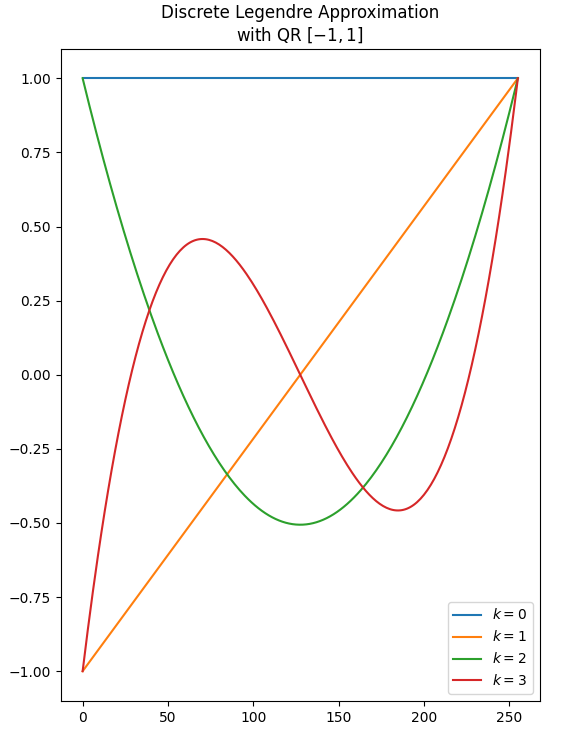
\includegraphics[width=0.5\textwidth]{vandermonde-qr-discrete-legendre-approximation}
			\caption{Exercise 9.1a: Discrete Legendre Polynomials Approximation for degrees $0$, $1$, $2$, $3$,  on the Interval $[-1,1]$ by finding the QR factorization of a Vandermonde matrix using $256$ grid points.}
			\label{fig:9.1a}
		\end{figure}
		\item See Figure~\ref{fig:9.1b} for a plot of the error, which I've computed as the difference of the
		exact values of the Legendre Polynomials on the same grid points minus the values of the approximation.
		The error is distributed symmetrically about 0 for each polynomial. Let $P_k$ denote the $k$th degree
		Legendre polynomial. The polynomials $P_0$ and $P_1$ match their approximations exactly. The errors in
		$P_2$ and $P_3$ show a symmetric graph. The error is greater away from their endpoints and near the relative
		extrema of the functions.
		\begin{figure}
			\centering
			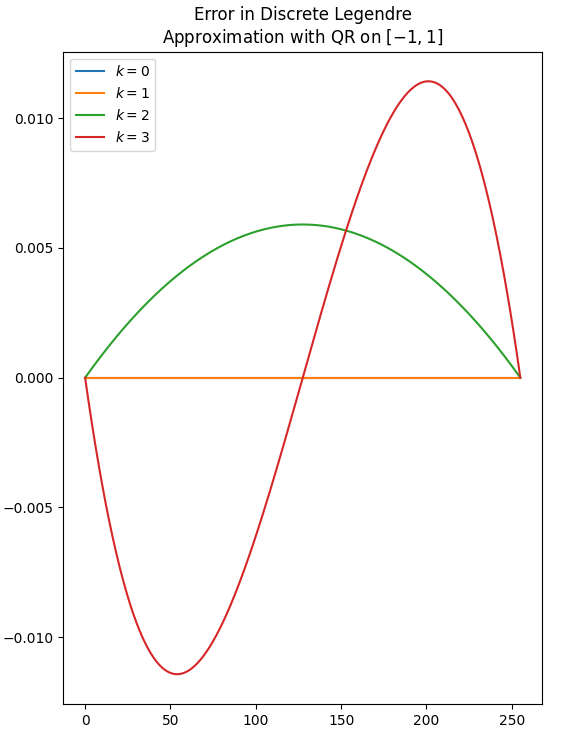
\includegraphics[width=0.6\textwidth]{error-in-discrete-legendre-approximation}
			\caption{Exercise 9.1b: Plot of error in approximation to Legendre Polynomials given in Figure~\ref{fig:9.1a},
				using $256$ grid points. Error is computed as the $P_{k, exact}(x)-P_{k, approx}$.}
			\label{fig:9.1b}
		\end{figure}
		\item I observed that an increase in the power of $\Delta x$  by 1 resulted in halving the maximum error
		across all polynomials.
	\end{enumerate}
\end{sol}

\begin{ex}{2}
	In Experiment 2, the singular values of $A$ match the diagonal elements of a QR factor $R$ approximately.
	Consider now a very different example. Suppose $Q=I$ and $A=R$, the $m\times m$ (a \emph{Toeplitz matrix})
	with 1 on the main diagonal, 2 on the first superdiagonal, and 0 everywhere else.
	\begin{enumerate}[label=(\alph*)]
		\item What are the eigenvalues, determinant, and rank of $A$?
		\item What is $A^{-1}$?
		\item Give a nontrivial upper bound on $\sigma_m$, the $m$th singular value for $A$. You are welcome
		to use MATLAB for inspiration, but the bound you give should be justified analytically.
		(\emph{Hint}: Use part (b).)
	\end{enumerate}
	This problem illustrates that you cannot always infer much about the singular values of a matrix
	form its eigenvalues or from the diagonal entries of a QR factor $R$
\end{ex}

\begin{sol}
	\
	\begin{enumerate}[label=(\alph*)]
		\item The \emph{superdiagonal} of a matrix is the set of elements above the elements comprising the
		diagonal (source: \href{https://mathworld.wolfram.com/Superdiagonal.html}{Wolfram}). Thus
		the matrix in question looks like:
		\begin{align*}
			A=R=\begin{bmatrix}
				1 & 2 & 0 & \cdots & \cdots & 0\\
				0 & 1 & 2 & 0 & \cdots & \vdots\\
				\vdots & 0 & \ddots& \ddots & \ddots & \vdots\\
				\vdots& \vdots & \vdots & \ddots & \ddots& 0\\
				\vdots & \vdots & \vdots & \vdots& \ddots & 2\\
				0 & 0 & \cdots & \cdots & 0 & 1
			\end{bmatrix}
		\end{align*}
		Since this matrix is upper-triangular, its eigenvalues are the values of its diagonal entries,
		all of which are 1. The determinant is the product of the diagonal entries, which is also 1.
		Finally, the rank of $A$ is $m$, because all of its eigenvalues are nonzero.
		\item The inverse is:
		\begin{align*}
			A^{-1}&=\begin{bmatrix}
				1 & -2 & 4& -8 & \cdots\\
				0 & 1 & -2& 4 & \cdots \\
				\vdots & 0 & 1 & -2 &\cdots\\
				\vdots & 0 & 0 & 1 & \cdots\\
				\vdots & \vdots &\vdots & 0 & \ddots
			\end{bmatrix}
		\end{align*}
		In other words, the inverse has 1s on the diagonal, $-2$ on the first super diagonal, $4$ on the next
		superdiagonal, $-8$ on the next superdiagonal, and so on.
		\item Note that if $A=U\Sigma V^*$ is a singular value decomposition of $A$, then
		$A^{-1}=V\Sigma^{-1}U^*$ is a singular value decomposition of $A^{-1}$. In other words,
		$\sigma_j$ is a nonzero singular value of $A$ if and only if $\frac{1}{\sigma_j}$ is a singular value
		of $A^{-1}$.
		
		Since $A\in\mathbb{C}^{m\times m}$ has invertible, all of its singular values are nonzero, so
		$\sigma_j>0$ for $j\in\{1,\ldots,m\}$. The singular values $\sigma_1,\ldots,\sigma_m$ are
		conventionally listed in descending order, meaning that $\sigma_1\geq \sigma_2\geq \cdots\sigma_m$.
		Thus, $\sigma_1$ is the value of the largest singular value  of $A$ and $\sigma_m$ is the value
		of the smallest singular value of $A$.
		
		
		By contrast, $\frac{1}{\sigma_1},\ldots,\frac{1}{\sigma_m}$ are the singular values of $A^{-1}$,
		but this is list is given in ascending order. In other words, the largest  singular value of
		$A^{-1}$ is $\frac{1}{\sigma_m}$. By Theorem 5.3, $\lVert A\rVert_2=\sigma_1$, where $\lVert\cdot\rVert_2$
		is vector-induced matrix 2-norm, and $\sigma_1$ is the largest singular value of $A$. Thus,
		applying the same Theorem to $A^{-1}$, we conclude that $\lVert A^{-1}\rVert_2 =\frac{1}{\sigma_m}$.
		
		Recall from Exercise 3.3(d) that $\lVert A^{-1}\rVert_\infty\leq \sqrt{m}\ \lVert A^{-1}\rVert_2$,
		where $\lVert \cdot \rVert_\infty$ is the vector-induced matrix $\infty$-norm.
		Let $(a^{-1}_k)^*$ denote the $k$-th row of $A^{-1}$, and recall also from Example 3.4 that
		$\lVert A^{-1}\rVert_\infty=\max_{1\leq k\leq m}\lVert (a^{-1}_k)^*\rVert_1$, where
		$\lVert \cdot\rVert_1$ is the vector $1$-norm. Then
		\begin{align*}
			\frac{1}{\sigma_m^2}&=\lVert A^{-1}\rVert_2\ ^2\\
			&\geq \frac{1}{m}\left\lVert A^{-1}\right\rVert_\infty\ ^2\\
			&=\frac{1}{m}\cdot \max_{1\leq i\leq m}\lVert (a_i^{-1})^*\rVert_1\\
			&=\frac{1}{m}\left(1^2 + |-2| + |4|^2+\cdot+|(-2)^{m-1}|\right)^2\\
			&=\frac{1}{m}\left(\cdot \sum_{k=0}^{m-1}2^k\right)^2\\
			&=\frac{1}{m}(2^m-1)^2
		\end{align*}
		Rearranging and taking square roots on both sides, we get $\frac{1}{m}(2^m-1)\geq \sigma_m$,
		and hence $\frac{1}{m}2^m$ is an upper bound of $\sigma_m$.
	\end{enumerate}
\end{sol}

\begin{ex}{3}
	\begin{enumerate}[label=(\alph*)]
		\item Write a MATLAB program that sets up a $15\times 40$ matrix with entries 0 everywhere except
		for the values $1$ in the positions indicated in the picture below. The upper-leftmost 1 is in
		position $(2,2)$, and the lower-rightmost $1$ is in position $(13,39)$. This picture was produced
		with the command \texttt{spy(A)}
		\item Call \texttt{svd} to compute the singular values of $A$, and print the results. Plot these
		numbers using both \texttt{plot} and \texttt{semilogy}. What is the mathematically exact rank of
		$A$? How does this show up in the computed singular values?
		\item For each $i$ from 1 to $\text{rank}(A)$, construct the rank-$i$ matrix $B$ that is the best
		approximation to $A$ in the $2$-norm. Use the command \texttt{pcolor(B)} with \texttt{colormap(gray)}
		to create images of these various approximations?
	\end{enumerate}
\end{ex}

\end{document}